\subsection{分次对偶 T(M)*gr、S(M)*gr 与 ∧(M)*gr}

从现在起，我们回到关于代数的章节的一般约定，因此（除非另有说明）假定这些代数是结合的且有单位的。

设 M 为一个 A-模；定义在 T(M)（第 1 号，例 5）、S(M)（第 1 号，例 6）和 \(\bigwedge\) (M)（第1号，例7）上的分次 A-余代数结构，依据第 2 号的命题 1 和命题 3 以及关于分次模的分次对偶的分次所作的约定（第 1 号），使我们能够典范地在分次对偶 T(M)*gr、S(M)*gr 和 \(\bigwedge\) (M)*gr 上定义 N 型分次代数结构。此外，分次代数 S(M)*gr 是交换的（第 2 号，命题 2 和例 5），且分次代数 \(\bigwedge\) (M)*gr 是反交换的（第3号，命题6及例）。在 \(\bigwedge\) (M)*gr 中，每个次数为 1 的元素的平方为零；这样的元素等同于 M 上的一个线性形式 \(f\) ，其平方是交错双线性形式 \(f \wedge f\) （在 M \(^{2}\) 上），使得

\[
(f \wedge f) (x, y) = f (x) f (y) - f (y) f (x)
\]

（第 2 号，例 3）。

设 \(\mathbf{N}\) 是另一个 A-模，且 \(u\) 为从 \(\mathbf{M}\) 到 \(\mathbf{N}\) 中的一个 A-线性映射。我们知道 \(u\) 典范地定义分次代数同态

\[
\left\{ \begin{array}{l} \mathsf {T} (u): \mathsf {T} (\mathbf {M}) \to \mathsf {T} (\mathbf {N}) \\ \mathsf {S} (u): \mathsf {S} (\mathbf {M}) \to \mathsf {S} (\mathbf {N}) \\ \bigwedge (u): \bigwedge (\mathbf {M}) \to \bigwedge (\mathbf {N}) \end{array} \right.\tag{23}
\]

（§ 5，第 2 号，§ 6，第 2 号和 § 7，第 2 号）。由第 1 号的公式 (3) 可立即验证 \(\mathsf{T}(u)\) 也是余代数态射。另一方面，若 \(\Delta_{\mathbf{M}}\) （相应地 \(\Delta_{\mathbf{N}}\) ）

表示对角映射 \(\mathbf{M} \to \mathbf{M} \times \mathbf{M}\) （相应地 \(\mathbf{N} \to \mathbf{N} \times \mathbf{N}\) ），则有关系式 \((u \times u) \circ \Delta_{\mathbf{M}} = \Delta_{\mathbf{N}} \circ u\) ；由此可得 \(\mathbf{S}(u \times u) \circ \mathbf{S}(\Delta_{\mathbf{M}}) = \mathbf{S}(\Delta_{\mathbf{N}}) \circ \mathbf{S}(u)\)

\[
(\text { resp. } \bigwedge (u \times u) \circ \bigwedge (\Delta_ {\mathbf {M}}) = \bigwedge (\Delta_ {\mathbf {N}}) \circ \bigwedge (u)).
\]

利用 \(\mathsf{S}(\mathbf{M})\) 和 \(\bigwedge (\mathbf{M})\) 中余积的定义（第 1 号，例 6 和 7）以及典范同构的函子性质，

\[
\mathbf {S} (\mathbf {M} \times \mathbf {M}) \rightarrow \mathbf {S} (\mathbf {M}) \otimes_ {\mathbf {A}} \mathbf {S} (\mathbf {M})
\]

和 \(\bigwedge (\mathbf{M}\times \mathbf{M})\to \bigwedge (\mathbf{M})^{\mathfrak{g}}\otimes_{\mathbf{A}}\bigwedge (\mathbf{M})\) ，可以看出 \(S(u)\) 和 \(\bigwedge (u)\) 也是余代数态射†（因此在这种情况下是双代数态射）。由此立即得出同态 (23) 的分次转置（II，§ 11，第 6 号）

\[
\begin{array}{c} ^ {t} \mathsf {T} (u): \mathsf {T} (\mathbf {N}) ^ {* \mathrm{gr}} \to \mathsf {T} (\mathbf {M}) ^ {* \mathrm{gr}} \\ ^ {t} \mathsf {S} (u): \mathsf {S} (\mathbf {N}) ^ {* \mathrm{gr}} \to \mathsf {S} (\mathbf {M}) ^ {* \mathrm{gr}} \\ ^ {t} \bigwedge (u): \bigwedge (\mathbf {N}) ^ {* \mathrm{gr}} \to \bigwedge (\mathbf {M}) ^ {* \mathrm{gr}} \end{array}
\]

是分次代数同态。

我们现在注意到，M 的对偶 M* 与 T(M)*gr（相应地，S(M)*gr，∧(M)*gr）中次数为 1 的元素所构成的子模等同。因此，由张量代数的泛性质（§ 5，第 1 号）和对称代数的泛性质（§ 6，第 1 号）可知，存在且仅存在一个分次代数同态

\[
\theta_ {\mathsf {T}}: T (M ^ {*}) \rightarrow T (M) ^ {* \mathrm{gr}}
\]

它延拓了典范单射 \(\mathbf{M}^{*}\to \mathsf{T}(\mathbf{M})^{*\mathrm{gr}}\) ，并且存在唯一一个分次代数同态

\[
\theta_ {\mathsf {S}}: S (M ^ {*}) \rightarrow S (M) ^ {* \mathrm{gr}}
\]

它延拓了典范单射 \(\mathbf{M}^{*}\to\mathsf{S}(\mathbf{M})^{*\mathrm{gr}}\) 。另一方面， \(\mathbf{M}^{*}\) 在 \(\bigwedge(\mathbf{M})^{*\mathrm{gr}}\) 的反代数中的典范单射使得 \(\mathbf{M}^{*}\) 的每个元素的平方为零；因此（§ 7，第 1 号，命题 1）存在唯一一个分次代数同态

\[
\theta_ {\wedge}: \bigwedge (\mathbf {M} ^ {*}) \rightarrow (\bigwedge (\mathbf {M}) ^ {* \mathrm{gr}}) ^ {\circ}
\]

它延拓了典范单射 \(M^{*}\to\bigwedge(M)^{*gr.}\) 。这些同态是函子性的：例如，对于每个 A-模同态 \(u:M\to N\) ，该图表

\pandocbounded{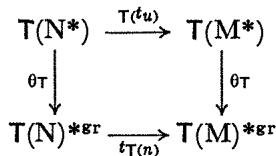
\includegraphics[keepaspectratio]{images/part004_1f4c9f33.jpg}}

是交换的，这直接从张量代数的泛性质（§ 5，第 1 号）得出；对 \(\theta_{s}\) 和 \(\theta_{\wedge}\) 也有类似的交换图。

我们将明确找出同态 \(\theta_{\mathsf{T}}\) , \(\theta_{\mathsf{S}}\) 和 \(\theta_{\wedge}\) 。为此，我们更一般地考虑一个带余积 \(c\) 的余结合 A-余代数 E，并对 \(n\) （ \(n \geqslant 2\) ）归纳地定义线性映射 \(c_{n}\) （从 E 到 \(\mathrm{E}^{\otimes n}\) 中），由 \(c_{2} = c\) 和

\[
c _ {n} = \left(c _ {n - 1} \otimes 1 _ {\mathrm{E}}\right) \circ c.\tag{24}
\]

另一方面，我们用 \(m_{n}:A^{\otimes n}\to A\) 表示典范线性映射，使得 \(m_{n}(\xi_{1}\otimes\xi_{2}\otimes\cdots\otimes\xi_{n})=\xi_{1}\xi_{2}\ldots\xi_{n}\) ，并注意，对 \(n\geqslant2\) ，

\[
m _ {n} = m \circ (m _ {n - 1} \otimes 1 _ {\mathbf {A}})\tag{25}
\]

记 \(m = m_2\) 。利用此记号：

引理1. (i) 在结合代数 \(\mathbf{E}^* = \operatorname{Hom}_{\mathbf{A}}(\mathbf{E}, \mathbf{A})\) 中， \(n\) 个 1 次元素 \(u_1, u_2, \ldots, u_n\) 的乘积由

\[
u _ {1} u _ {2} \dots u _ {n} = m _ {n} \circ (u _ {1} \otimes u _ {2} \otimes \dots \otimes u _ {n}) \circ c _ {n}.\tag{26}
\]

\begin{enumerate}
\def\labelenumi{(\roman{enumi})}
\setcounter{enumi}{1}
\tightlist
\item
  还假设余代数 E 是分次的。那么，在分次结合代数 \(\mathbf{E}^{*\mathrm{gr}} = \operatorname{Homgr}_{\mathbf{A}}(\mathbf{E}, \mathbf{A})\) 中， \(n\) 个 1 次元素 \(u_1, u_2, \ldots, u_n\) 的乘积由
\end{enumerate}

\[
u _ {1} u _ {2} \dots u _ {n} = m _ {n} \circ (u _ {1} \otimes u _ {2} \otimes \dots \otimes u _ {n}) \circ \delta_ {n}\tag{27}
\]

（其中 \(\delta_n: \mathbf{E} \to \mathbf{E}^{\otimes n}\) 是把每个 \(x \in \mathbf{E}\) 映为 \(c_n(x)\) 的多重次数 \((1, 1, \ldots, 1)\) 分量的线性映射。

公式（26）正是 \(\mathbf{E}^*\) 中乘积在 \(n = 2\) 时的定义；要对 \(n\) 用归纳法证明它，观察到

\[
\begin{array}{l} u _ {1} u _ {2} \dots u _ {n} \\ \qquad = m \circ ((u _ {1} u _ {2} \dots u _ {n - 1}) \otimes u _ {n}) \circ c \\ \qquad = m \circ ((m _ {n - 1} \circ (u _ {1} \otimes u _ {2} \otimes \dots \otimes u _ {n - 1}) \circ c _ {n - 1}) \otimes u _ {n}) \circ c \\ \qquad = m \circ (m _ {n - 1} \otimes \mathrm{l} _ {\mathrm{A}}) \circ (u _ {1} \otimes u _ {2} \otimes \dots \otimes u _ {n - 1} \otimes u _ {n}) \circ (c _ {n - 1} \otimes \mathrm{l} _ {\mathrm{E}}) \circ c \\ \qquad = m _ {n} \circ (u _ {1} \otimes u _ {2} \otimes \dots \otimes u _ {n}) \circ c _ {n} \end{array}
\]

根据（24）、（25）、II，§3，第3号，公式（5）以及关系式

\[
u _ {n} = 1 _ {\mathbf {A}} \circ u _ {n} \circ 1 _ {\mathbf {E}}.
\]

当 E 是分次的且元素 \(u_{i} \in E^{*gr}\) 是 1 次齐次的时，根据定义，对齐次元素 \(x_{i} \in E\) ，

\[
(u _ {1} \otimes u _ {2} \otimes \dots \otimes u _ {n}) (x _ {1} \otimes x _ {2} \otimes \dots \otimes x _ {n}) = 0
\]

除非所有 \(x_{i}\) 的次数均为 1，由此得到公式 (27) 。

由第1号中的公式 (3)、(5)和(7)以及公式 (24) 可知，当 E 取为三个分次余代数 \(\mathsf{T}(\mathbf{M})\) , \(\mathsf{S}(\mathbf{M})\) 和 \(\bigwedge (\mathbf{M})\) 之一时，对 \(n\) 用归纳法（利用余积是次数为 0 的分次同态这一事实）分别得到，对 M 中的 \(x_{1}, x_{2}, \ldots, x_{n}\) ：

\[
\text { when   } \mathrm{E} = \mathrm{T} (\mathrm{M}), \quad \delta_ {n} (x _ {1} x _ {2} \dots x _ {n}) = x _ {1} \otimes x _ {2} \otimes \dots \otimes x _ {n}
\]

\[
\text { when } \mathrm{E} = \mathrm{S(M)}, \quad \delta_ {n} (x _ {1} x _ {2} \dots x _ {n}) = \sum_ {\sigma \in \mathfrak {S} _ {n}} x _ {\sigma (1)} \otimes x _ {\sigma (2)} \otimes \dots \otimes x _ {\sigma (n)}
\]

\[
\text { when } \mathrm{E} = \bigwedge (\mathrm{M}), \quad \delta_ {n} (x _ {1} x _ {2} \dots x _ {n}) = \sum_ {\sigma \in \mathfrak {S} _ {n}} \varepsilon_ {\sigma}. x _ {\sigma (1)} \otimes x _ {\sigma (2)} \otimes \dots \otimes x _ {\sigma (n)}.
\]

只需注意，例如当 \(\mathbf{E} = \bigwedge (\mathbf{M})\) 时，在由第1号公式 (8) 得出的表达式 \(c_{n}(x_{1}x_{2}\ldots x_{n}) = (c_{n - 1}\otimes 1_{\mathbb{E}})\left(\sum (-1)^{\nu}(x_{i_1}\ldots x_{i_p})\otimes (x_{j_1}\ldots x_{j_{n - p}})\right)\) 中，唯一能给出多重次数 \((1,1,\dots ,1)\) 项的是那些使 \(n - p = 1\) 的项，因此

\[
\delta_ {n} (x _ {1} x _ {2} \dots x _ {n})
\]

是以下和中多重次数为 \((1, 1, \ldots, 1)\) 的项

\[
\sum_ {i = 1} ^ {n} (- 1) ^ {n - i} c _ {n - 1} \left(x _ {1} \dots x _ {i - 1} x _ {i + 1} \dots x _ {n}\right) \otimes x _ {i}
\]

且这一项必然等于

\[
\sum_ {i = 1} ^ {n} (- 1) ^ {n - i} \delta_ {n - 1} (x _ {1} \dots x _ {i - 1} x _ {i + 1} \dots x _ {n}) \otimes x _ {i},
\]

因此由归纳假设可得结果。

根据引理1， \(\mathsf{T}(\mathbf{M})^{*\mathrm{gr}}\) 中 \(n\) 个线性形式 \(x_{1}^{*}, x_{2}^{*}, \ldots, x_{n}^{*}\) （属于 \(\mathbf{M}^{*}\) ）的乘积由以下公式给出

\[
\left\langle x _ {1} ^ {*} x _ {2} ^ {*} \dots x _ {n} ^ {*}, x _ {1} x _ {2} \dots x _ {n} \right\rangle = \prod_ {i = 1} ^ {n} \left\langle x _ {i} ^ {*}, x _ {i} \right\rangle\tag{28}
\]

对 \(x_{i} \in \mathbf{M} (1 \leqslant i \leqslant n)\) 成立；这 \(n\) 个形式在 \(S(M)^{*gr}\) 中的乘积由以下公式给出

\[
\left\langle x _ {1} ^ {*} x _ {2} ^ {*} \dots x _ {n} ^ {*}, x _ {1} x _ {2} \dots x _ {n} \right\rangle = \sum_ {\sigma \in \mathfrak {S} _ {n}} \left(\prod_ {i = 1} ^ {n} \left\langle x _ {\sigma (i)} ^ {*}, x _ {i} \right\rangle\right);\tag{29}
\]

最后，这些形式在 \(\bigwedge (\mathbf{M})^{*\mathrm{gr}}\) 中的乘积由以下公式给出

\[
\langle x _ {1} ^ {*} x _ {2} ^ {*} \dots x _ {n} ^ {*}, x _ {1} x _ {2} \dots x _ {n} \rangle = \det (\langle x _ {i} ^ {*}, x _ {j} \rangle).\tag{30}
\]

在三种情形中，我们分别有

\[
\theta_ {T} (x _ {1} ^ {*} \otimes x _ {2} ^ {*} \otimes \dots \otimes x _ {n} ^ {*}) = x _ {1} ^ {*} x _ {2} ^ {*} \dots x _ {n} ^ {*}
\]

\[
\theta_ {S} (x _ {1} ^ {*} x _ {2} ^ {*} \dots x _ {n} ^ {*}) = x _ {1} ^ {*} x _ {2} ^ {*} \dots x _ {n} ^ {*}
\]

\[
\theta_ {\wedge} (x _ {1} ^ {*} \wedge x _ {2} ^ {*} \wedge \dots \wedge x _ {n} ^ {*}) = x _ {n} ^ {*} x _ {n - 1} ^ {*} \dots x _ {1} ^ {*} = (- 1) ^ {n (n - 1) / 2} x _ {1} ^ {*} x _ {2} ^ {*} \dots x _ {n} ^ {*}
\]

因此，我们从 (28)、(29) 和 (30) 推导出以下关系式

\[
\langle \theta_ {T} (x _ {1} ^ {*} \otimes x _ {2} ^ {*} \otimes \dots \otimes x _ {n} ^ {*}), x _ {1} \otimes x _ {2} \otimes \dots \otimes x _ {n} \rangle = \prod_ {i = 1} ^ {n} \langle x _ {i} ^ {*}, x _ {i} \rangle\tag{28 bis}
\]

（换言之， \(\theta_{\mathsf{T}}\) 在 \(\mathsf{T}^2 (\mathbf{M}^*)\) 上的限制就是 II，§4，第4号中的典范同态）

\[
\langle \theta_ {\mathsf {S}} (x _ {1} ^ {*} x _ {2} ^ {*} \dots x _ {n} ^ {*}), x _ {1} x _ {2} \dots x _ {n} \rangle = \sum_ {\sigma \in \mathfrak {S} _ {n}} \left(\prod_ {i = 1} ^ {n} \langle x _ {\sigma (i)} ^ {*}, x _ {i} \rangle\right)\tag{29 bis}
\]

\[
\begin{array}{r l} (30 \text { bis}) &\langle \theta_ {\wedge} (x _ {1} ^ {*} \wedge x _ {2} ^ {*} \wedge \dots \wedge x _ {n} ^ {*}), x _ {1} \wedge x _ {2} \wedge \dots \wedge x _ {n} \rangle \\ & \qquad = (- 1) ^ {n (n - 1) / 2} \mathrm{det} (\langle x _ {i} ^ {*}, x _ {j} \rangle). \end{array}
\]

命题7. 设 \(\mathbf{M}\) 是有限生成的投射 A-模。则典范同态 \(\theta_{\mathsf{T}}: \mathsf{T}(\mathbf{M}^{*}) \to \mathsf{T}(\mathbf{M})^{*\mathrm{gr}}\) 和 \(\theta_{\wedge}: \bigwedge (\mathbf{M}^{*}) \to (\bigwedge (\mathbf{M})^{*\mathrm{gr}})^{0}\) 是双射。此外，分次对偶 \(\bigwedge (\mathbf{M})^{*\mathrm{gr}}\) 此时等于对偶 \(\bigwedge (\mathbf{M})^{*}\) ，即 A-模 \(\bigwedge (\mathbf{M})\) 的对偶。

首先假设 \(\mathbf{M}\) 具有有限基 \((e_i)_{1\leq i\leq m}\) ，并设 \((e_i^*)_{1\leq i\leq m}\) 为 \(\mathbf{M}^*\) 的对偶基 (II, § 10, no. 4)。公式 (28 bis) 表明，对每个有限序列 \(s = (j_k)_{1\leq k\leq n}\) （ \(n\) 个元素取自区间 \([1,m]\) （ \(\mathbf{N}\) 的）），

\[
\theta_ {\mathsf {T}} (e _ {j _ {1}} ^ {*} \otimes \dots \otimes e _ {j _ {n}} ^ {*})
\]

是指标为 \(s\) 的元素，位于 \((\mathsf{T}^n (\mathbf{M}))^*\) 的基中，该基对偶于 \(\mathsf{T}^n (\mathbf{M})\) 的由 \(e_s = e_{j_1}\otimes \dots \otimes e_{j_n}\) 组成的基（§ 5，第 5 号，定理 1）。因此 \(\theta_{\mathsf{T}}\) 是双射。

类似地，公式（30 bis）表明，对每个有限子集 \(\mathbf{H}\) （属于 \([1, m]\) ，含 \(n\) 个元素）， \((-1)^{n(n-1)/2} \theta_{\wedge}(e_{\mathrm{H}}^{*})\) （§7，第8号，定理1的记号）是指标为 \(\mathbf{H}\) 的元素，位于 \((\bigwedge^{n}(\mathbf{M}))^{*}\) 的基中，该基对偶于 \(\bigwedge^{n}(\mathbf{M})\) 的由 \(e_{\mathrm{H}}\) 组成的基。因此 \(\theta_{\wedge}\) 是双射。

现在仅假设 M 是有限生成且投射的；则 M 是有限生成自由 A-模 L 的一个直和因子，因此存在两个

A-线性映射 \(M \xrightarrow{j} L \xrightarrow{p} M\) ，其复合为恒等映射 \(1_{M}\) 。由此我们推导出一个交换图

\pandocbounded{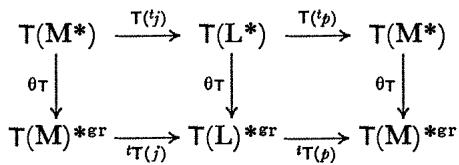
\includegraphics[keepaspectratio]{images/part004_2d3cbe02.jpg}}

以及一个类似的交换图，其中 \(\mathsf{T}\) 被替换为 \(\bigwedge\) 。该命题随后由以下引理得出：

引理2. 设

\pandocbounded{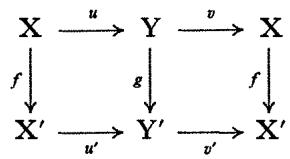
\includegraphics[keepaspectratio]{images/part004_a09507a7.jpg}}

是一个集合与映射的交换图，使得 \(v \circ u\) 和 \(v' \circ u'\) 分别是 \(X\) 和 \(X'\) 的恒等映射。那么，若 \(g\) 是单射（相应地，满射、双射），则 \(f\) 亦然。

u 是单射，因为 \(v \circ u\) 是；因此，若 g 是单射， \(u' \circ f = g \circ u\) 是单射，从而 f 是单射。类似地 \(v'\) 是满射，因为 \(v' \circ u'\) 是；因此，若 g 是满射， \(f \circ v = v' \circ g\) 是满射，从而 f 是满射。

命题7的最后断言由以下事实得出： \(\bigwedge (\mathbf{M})\) 此时是一个有限生成的 A-模（§ 7，第 3 号，命题 6 及 II，§ 11，第 6 号，注记）。

我们现在考察关于同态 \(\theta_{\mathsf{S}}\) （当 \(\mathbf{M}\) 是投射的且有限生成时）可以说些什么。首先假设 \(\mathbf{M}\) 具有有限基 \((e_i)_{1\leq i\leq m}\) 。在本章开头的记号中，A-模 \(\mathbf{S}^n (\mathbf{M})\) 以元素族 \(e^{\alpha}\) （满足 \(|\alpha | = n\) ）为基。设 \(u_{\alpha}\) （对于 \(|\alpha | = n\) ）表示指标为 \(\alpha\) 的元素，位于 \((\mathbf{S}^n (\mathbf{M}))^*\) 的对偶于 \((e^{\alpha})\) 的基中。元素 \(u_{\alpha}\) （对于 \(\alpha \in \mathbf{N}^m\) ）因此构成代数 \(\mathbf{S}(\mathbf{M})^{*\mathrm{gr}}\) 的基，我们将显式给出这个基的乘法表。我们记

\[
u _ {\alpha} u _ {\beta} = \sum_ {\gamma \in \mathbf {N} ^ {m}} a _ {\alpha \beta \gamma} u _ {\gamma} \quad \text { with } a _ {\alpha \beta \gamma} \in \mathrm{A}.
\]

那么根据定义

\[
a _ {\alpha \beta \gamma} = \langle u _ {\alpha} u _ {\beta}, e ^ {\gamma} \rangle = m ((u _ {\alpha} \otimes u _ {\beta}) (c (e ^ {\gamma}))),
\]

（其中 \(m: \mathbf{A} \otimes \mathbf{A} \to \mathbf{A}\) 定义 \(\mathbf{A}\) 上的乘法， \(c\) 是 \(\mathsf{S}(\mathbf{M})\) 的余积。换言之， \(a_{\alpha \beta \gamma}\) 正是 \(e^{\alpha} \otimes e^{\beta}\) 的系数（当 \(c(e^{\gamma})\) 用 \(\mathsf{S}(\mathbf{M})\otimes \mathsf{S}(\mathbf{M})\) 的由 \(e^{\xi}\otimes e^{\eta}\) 组成的基表示时），其中 \(\xi\) 和 \(\eta\) 遍历 \(\mathbf{N}^m\) 。但由于 \(c\) 是代数同态，

\[
c (e ^ {\gamma}) = \prod_ {i = 1} ^ {m} (c (e _ {i})) ^ {\gamma_ {i}} = \prod_ {i = 1} ^ {m} (e _ {i} \otimes 1 + 1 \otimes e _ {i}) ^ {\gamma_ {i}}
\]

根据第1号公式 (4)，这给出

\[
c (e ^ {\gamma}) = \sum_ {\xi + \eta = \gamma} (\xi , \eta) e ^ {\xi} \otimes e ^ {\eta}\tag{31}
\]

其中我们记

\[
((\xi , \eta)) = \prod_ {i = 1} ^ {n} \frac {(\xi_ {i} + \eta_ {i}) !}{\xi_ {i} ! \eta_ {i} !} \quad (\text { cf.   } \S 10, \text {   no.   } 4, \text {   formula   (18) }).\tag{32}
\]

因此我们得到乘法表

\[
u _ {\alpha} u _ {\beta} = ((\alpha , \beta)) u _ {\alpha + \beta}.\tag{33}
\]

另一方面，如果 \((e_i^*)_{1\leq i\leq m}\) 是 \(\mathbf{M}^*\) 的、对偶于 \((e_i)\) 的基，则由公式 (29 bis) 可知，对所有 \(\alpha \in \mathbf{N}^m\) ，

\[
\theta_ {S} (e ^ {* \alpha}) = \alpha ! u _ {\alpha}\tag{34}
\]

在 §6 第6号的记号中。因此同态 \(\theta_{\mathsf{S}}\) 是双射当且仅当诸 \(\alpha!u_{\alpha}\) 构成 \(\mathsf{S}(\mathbf{M})^{*\mathrm{gr}}\) 的一组基，亦即诸元素 \(\alpha!1\) 均可逆。

命题8. 假设环 A 是有理数域 Q 上的代数；那么，对于每个有限生成的投射 A-模 M，同态

\[
\theta_ {\mathsf {S}}: S (M ^ {*}) \rightarrow S (M) ^ {* \mathrm{gr}}
\]

是双射。

这相当于在M有限生成且自由的情形下证明；我们像命题7的证明中那样，利用引理2从这一情形过渡到一般情形。

注记。设 M 为一个 A-模，且 \(\rho: \mathbf{A} \to \mathbf{B}\) 为一个交换环同态。则存在一个分次 B-代数同态的交换图

\[
\begin{array}{l} \mathsf {T} ((\mathbf {M} ^ {*}) _ {(B)}) \longrightarrow (\mathsf {T} (\mathbf {M}) ^ {* \mathrm{gr}}) _ {(B)} \\ \mathsf {T} (\upsilon_ {\mathbf {M}}) \Biggl \downarrow \qquad \qquad \qquad \qquad \qquad \qquad \qquad \qquad \qquad \Biggl \downarrow \upsilon_ {\mathbf {T} (\mathbf {M})} \\ \mathsf {T} ((\mathbf {M} _ {(B)}) ^ {*}) \xrightarrow [ \theta_ {\mathsf {T}} ]{} \mathsf {T} (\mathbf {M} _ {(B)}) ^ {* \mathrm{gr}} \end{array}
\]

其中第一行是由同态 \(\theta_{\mathsf{T}}\otimes 1_{\mathsf{B}}\colon \mathsf{T}(\mathbf{M}^{*})\otimes_{\mathbf{A}}\mathbf{B}\to \mathsf{T}(\mathbf{M})^{*\mathrm{gr}}\) 与典范同构

\[
\mathsf {T} ((\mathbf {M} ^ {*}) _ {(\mathbf {B})}) \rightarrow \mathsf {T} (\mathbf {M} ^ {*}) \otimes_ {\mathbf {A}} \mathbf {B}
\]

（§ 5，第 3 号，命题 5）复合而成的同态。利用公式 (28) 及同态 \(\upsilon_{\mathbf{E}}\) （II，§ 5，第 4 号）的定义，可立即验证此图表是交换的。当 \(\mathbf{M}\) 是有限生成的投射 A-模时， \(\mathbf{M}_{(\mathbf{B})}\) 是有限生成的投射 B-模（II，§ 5，第 1 号，命题 4 的推论），且上述图表中的所有同态都是双射（命题 7 及 II，§ 5，第 4 号，命题 8）。存在类似的交换图，其中 \(\mathsf{T}\) 被替换为 \(\mathsf{S}\) 或 \(\bigwedge\) ；关于 \(\bigwedge\) 的那个图当 \(\mathbf{M}\) 是投射的且有限生成时也由双射同态组成（命题 7）；若进一步 \(\mathbf{A}\) 是 \(\mathbf{Q}\) 上的代数，则关于 \(\mathsf{S}\) 的图也由双射同态组成（命题 8）。

